\documentclass[../main.tex]{subfiles}
\graphicspath{{\subfix{../images/}}}

\begin{document}

\hypertarget{vulnerability-detection-module}{%
\chapter{The Vulnerability Detection
Module}\label{vulnerability-detection-module}}

The vulnerability detection module's \cite{vulnerability_detection_module_repo} objective is to uncover
vulnerabilities in executables using the information retrieved by the
attack surface approximation module (the input streams, arguments, and
their responsibilities). This approach not only concludes the
probability of a vulnerability occurring, but it also generates an
actual proof of vulnerability (i.e.~an input that triggers the
vulnerability) object, \texttt{ProofOfVulnerability}. It will then be
provided outside the module, namely to the vulnerability analytics
module, to obtain the root cause and the affected executable internals.

Even though this chapter only discusses fuzzing to find vulnerabilities, \cite{bogdan} discusses merging symbolic execution with Retdec\simplefootnote{https://github.com/avast/retdec} and KLEE\simplefootnote{https://github.com/klee/klee} in this
OpenCRS module.

\hypertarget{theoretical-considerations}{%
\section{Theoretical Considerations}\label{theoretical-considerations}}

Path explosion, a problem particular to approaches such as symbolic
execution, can arise during the investigation of the executable and its
execution. Because symbolic values are propagated down each path of the
graph, the complexity of detecting vulnerabilities in such a vast
quantity of data is impractical given memory and compute capacity
constraints.

We then use fuzzing to get around this. The sending of random inputs on
each input stream causes the execution to go in different directions,
with different input variables. The likelihood of triggering a
vulnerability could then be raised.

Another major constraint for fuzzing is the CRS's black-box (or
binary-only) nature: the vulnerability discovery module does not have
access to the executable's source code, but only to the binary itself.
This narrowed our search because fuzzers usually use source code
instrumentation, which involves inserting small amounts of code during
the compilation stage so that the fuzzer can determine which path of the
control flow graph was reached by the execution.

To begin, we investigated American Fuzzy Lop (AFL) \cite{afl} as a cutting-edge
blackbox fuzzer that we could integrate into the cyber reasoning system,
but Google's upstream has had no development activity since June 2021,
and the repository itself is archived. A possible alternative is afl++ \cite{aflpp},
a fork of it that is constantly developed by the open-source community
and offers features such as:

\begin{landscape}
\vspace*{\fill}
\begin{figure}[!h]
   \centering
    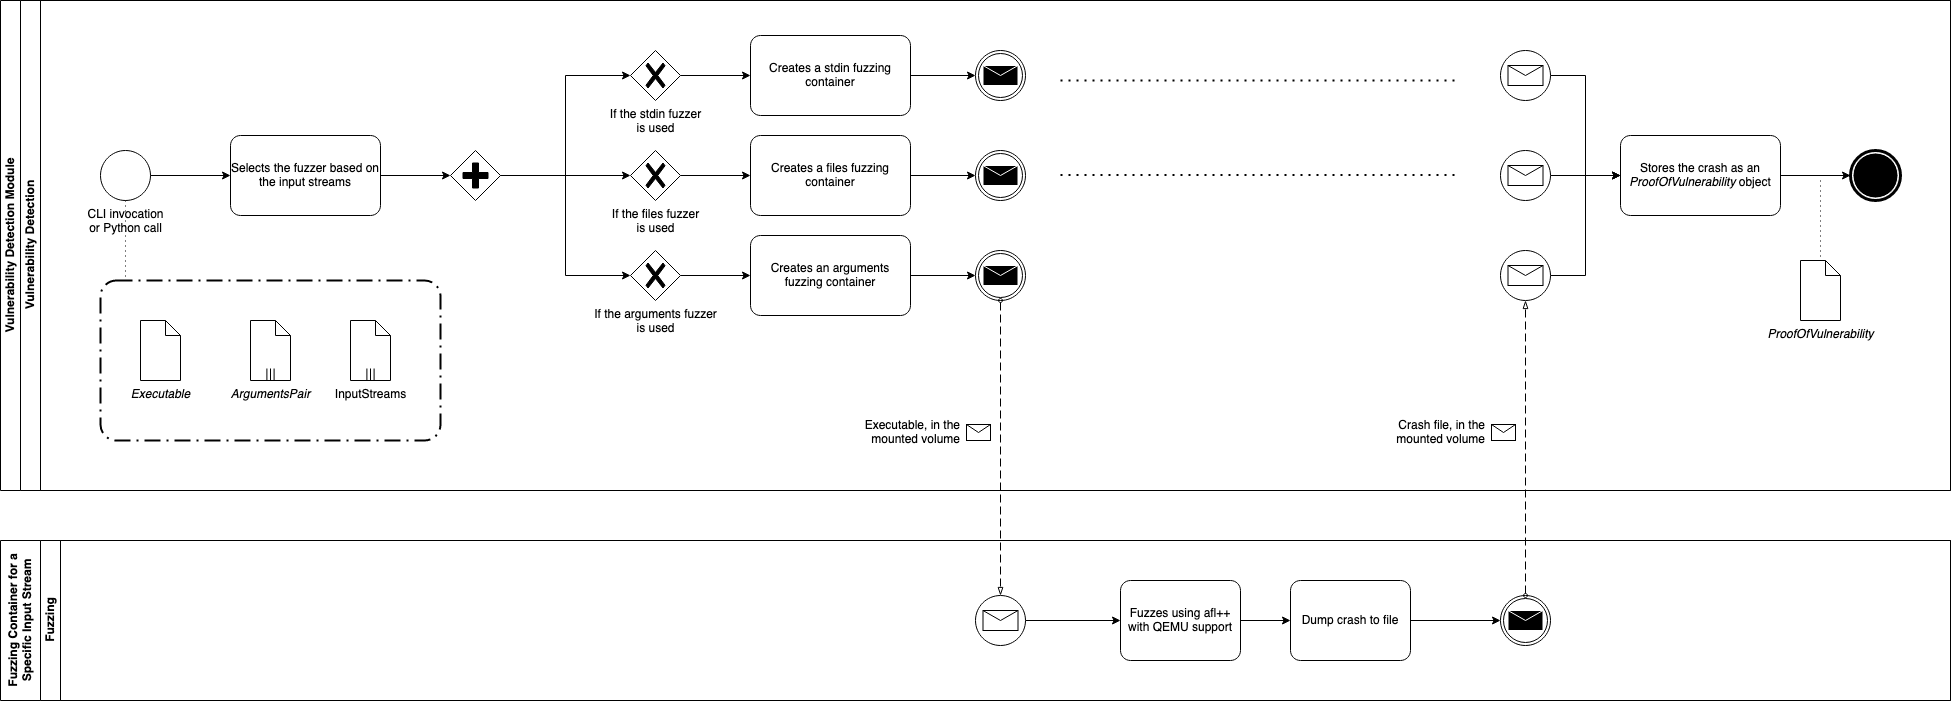
\includegraphics[width=0.95\linewidth]{images/vuln.png}
    \caption{Architecture of the Vulnerability Detection Module}
    \label{fig:vuln_architecture}
\end{figure}
\vspace*{\fill}
\end{landscape}

\begin{itemize}
\tightlist
\item
  QEMU emulation for deducing relevant information (for example,
  coverage) on runtime, without the need for source code instrumentation
  prior to compilation;
\item
  Persistent mode for specifying a section of the code segment that
  should be executed in a loop by the fuzzer, without the need to create
  a process each time new inputs are provided to the executable; and
\item
  Increased speed, resulting in more mutations in the fuzzing engine.
\end{itemize}

\hypertarget{implementation}{%
\section{Implementation}\label{implementation}}

Our method began by evaluating a subset of all possible input streams
(files, standard input, and arguments) that an executable could have.
When calling the vulnerability detection functionality, this information
is explicitly provided, and it can be derived using the attack surface
approximation module.

As previously stated, afl++ was chosen as a tool for blackbox fuzzing.
We designed a custom Docker image to serve as its environment, with the
aims of isolation and easy regeneration in mind. QEMU support for
binary-only fuzzing was enabled by running the
\texttt{build\_qemu\_support.sh} script.

It is instantiated by utilizing the Docker API for Python, with the
necessary volumes (for target executable, sample inputs, and analysis)
automatically attached. Furthermore, the same Python code runs
\texttt{afl-fuzz} inside the newly constructed container to fuzz the
supplied target executable with the sample inputs (if any). These are
mutated and given to standard input or placed in files (afl++ supports
two input streams by default), data that is consumed by the binary.

When afl++ detects a new crash for \texttt{stdin} and files, it creates
a new file in the analysis directory
(\texttt{/tmp/fuzzer/<session>/output/default/crashes/}),
which is continuously watched by a Python watchdog. The crash file is
read in order to construct a new instance of the
\texttt{ProofOfVulnerability} class.

For argument fuzzing, we utilized the same Docker image. The primary
difference is that the fuzzed binary is no longer the target binary, but
rather a customized adaptor written in C. The wrapper reads from
\texttt{stdin} the random input created by afl++. The input is then
tokenized by utilizing space as a delimiter (\texttt{0x20} ASCII) and
detecting formatting placeholders (\texttt{\%s}) that it replaces with
the input generated by afl++. The generated \texttt{char\ *} sequence is
passed as an \texttt{argv} argument to an \texttt{execve} call.

The adapter's image is the process's initial image as formed by the
fuzzer. Using the given approach, the system call substitutes the process
image with the actual target binary image, with a random string of
characters as parameters. Mismanagement of an argument can result in a
crash, which afl++ can identify and report to our watchdog.

\end{document}